\section{Zobrazenia}

Zobrazenia sa často nazývajú funkcie. Obe slová znamenajú to isté, obvykle však funkcia zobrazuje do čísel ($\mathbb{N}, \mathbb{R}, \mathbb{C}, \dots$).
Ktoré slovo sa použije je otázkou konvencie v danej časti matematiky.

\begin{definition}[zobrazenie]\label{def:zobrazenie}
Nech $A, B$ sú množiny.
\emph{Zobrazenie} $f$ z $A$ do $B$ je predpis, ktorý každému prvku
$A$ priradí nejaký prvok $B$.
Zapisujeme 
\[
f \colon A \to B.
\]
$A$ je \emph{definičný obor}, $B$ je \emph{koobor}.
\end{definition}

To znamená, že ak chceme špecifikovať nejaké zobrazenie $f$, musíme špecifikovať tri
veci:
\begin{enumerate}
    \item Z ktorej množiny sa zobrazuje (definičný obor).
    \item Do ktorej množiny sa zobrazuje (koobor).
    \item Predpis, ktorý nám určí, pre každý prvok definičného oboru ktorý prvok sa mu má zobraziť.
\end{enumerate}

Predpis môže byť daný rôzne.
Napríklad ak $f \colon \mathbb{R} \to \mathbb{R}$ môžeme predpis niekedy poznamenať pomocou vzorca, napr.
\[
f(x) = \sqrt{x^2+1}
\]
Ale $A, B$ vôbec nemusia byť množiny čísel, a predpis nemusí byť vzorec!
\begin{example}
Niekedy $A$ nemá číselnú povahu, $B$ áno.
\begin{itemize}
    \item $A = \text{všetky adresy v meste}$
    \item $B = \mathbb{R}$
\end{itemize}
Zobrazenie $d \colon A \to B$ môže byť \[
d(x) = \text{najkratšia vzdialenosť pri ceste peši medzi adresou $x$ a SvF STU, v minútach}.\]
Napríklad: $d(\text{moje bydlisko}) = 80$, $d(\text{Bernolákova 1})=8$.
\end{example}


\begin{example}
$g \colon \mathbb{N} \rightarrow \mathbb{N}$ dané predpisom $g(n) = n^2 + 1$.
Toto nám hovorí, že $g$ zobrazuje z množiny všetkých prirodzených čísel do množiny všetkých prirodzených čísel.
Predpis je teda v tomto prípade daný vzorcom, ktorý nám umožňuje počítať hodnoty zobrazenia pre konkrétne prvky definičného oboru $g$ (t.j. prirodzené čísla) dosadením a výpočtom.
\begin{align*}
    g(2) &= 2^2 + 1 = 5 \\
    g(7) &= 7^2 + 1 = 50
\end{align*}
$g(-1) = ?$ Toto neexistuje, pretože $-1 \notin \mathbb{N}$ a nie je to teda prvok definičného oboru $g$.
\end{example}

\begin{example}\label{ex:jedlo}
Nech $A = \{\text{Jožko, Miško}\}$ a $B = \{\text{bageta, guláš, jablko}\}$.
Nech $j \colon A \rightarrow B$ je zobrazenie "najobľúbenejšie jedlo".
V tomto prípade je definičný konečná množina.
Preto nám stačí napísať hodnotu
zobrazenia $j$ v každom prvku množiny $A$:
\begin{itemize}
    \item $f(\text{Jožko}) = \text{bageta}$
    \item $f(\text{Miško}) = \text{guláš}$
    \item $f(\text{Janka}) = \text{guláš}$
\end{itemize}

Zobrazenie $j$ môžeme aj nakresliť:
\begin{center}
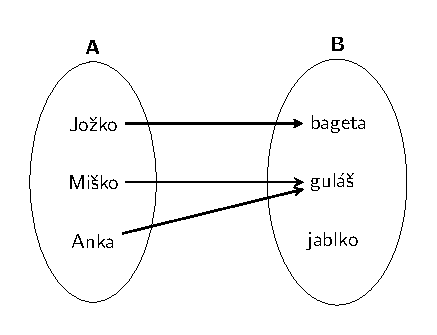
\includegraphics{figures/predn2_fig1.pdf}
\end{center}
\end{example}

Iný spôsob špecifikácie predpisu zobrazenia je napríklad tabuľkou:
\begin{center}
\begin{tabular}{c|ccc}
    $x$ & Jožko & Miško & Anka \\
    \hline
    $j(x)$ & bageta & guláš & guláš
\end{tabular}
\end{center}
Tu sa, samozrejme, nesmú prvky v hornom riadku opakovať.
\begin{example}
Nech $H$ je množina všetkých ľudí (aj z minulosti).
$\sigma \colon H \rightarrow H$ je zobrazenie dané predpisom $\sigma(x) = \text{otec človeka } x$.
\end{example}

\begin{example}
$S$ - množina všetkých občanov SR.
$\eta \colon S \rightarrow \mathbb{N}$ dané predpisom $\eta(x) = \text{rodné číslo}$.
\end{example}

\begin{example}
$B = \{\text{bageta, guláš, jablko}\}$. Nech $k \colon B \rightarrow \mathbb{R}$ je zobrazenie "koľko kalórií".
Keďže $B$ je konečná, stačí nám napísať:
$k(\text{guláš}) = 677$, $k(\text{bageta}) = 1148$, $k(\text{jablko}) = 301.4$.
\end{example}

\begin{example}
Poznáme nejaký príklad zobrazenia typu $A\times A\to A$, kde $A$ je nejaká množina? Samozrejme, už od prvého ročníka
základnej školy. Vezmime $A=\Nat$; sformulovať nejaký predpis pre zobrazenie 
$\Nat\times\Nat\to\Nat$ znamená povedať, ako vyrobiť z usporiadanej dvojice prirodzených čísel prirodzené
číslo. Napríklad môžeme definovať zobrazenie $+\colon A\times A\to A$ predpisom
\[
+(x,y)=\text{súčet čísel $x,y$}
\]
máme teda $+(1,3)=4$, $+(4,4)=8$. Samozrejme, zaužívaný spôsob zapisovania hodnoty zobrazenia $+$ v nejakej dvojici
$(a,b)\in\Nat\times\Nat$ je iný, nepíšeme obvykle $+(a,b)$, ale znak zobrazenia dáme medzi prvú a druhú zložku
usporiadanej dvojice, $a+b$. To je však detail, ktorý nič nemení na dôležitom náhľade, že sčítanie je zobrazením
z nejakej množiny do inej množiny.
\end{example}

Predošlý príklad je poučný v tom, že ukazuje ako jazyk postavený na pojmoch ,,množina'' a ,,zobrazenie'' umožňuje
popisovať matematické pojmy. Tento jazyk sa začal účinne používať na popis existujúcej a objavovanie novej matematiky v
20. storočí a dnes si už matematiku bez množín ani nevieme predstaviť.

Jeden zo spôsobov zapisovania zobrazení je ,,po prípadoch'', ako v nasledujúcich
dvoch príkladoch.
\begin{example}
\emph{Absolútna hodnota} je zobrazenie $\mathbb R\to\mathbb R$ dané predpisom
\[
|x|=
\begin{cases}
x& x\geq 0\\
-x& x<0
\end{cases}
\]
\end{example}
\begin{example}
\emph{Znamienková funkcia} alebo \emph{signum} je zobrazenie 
$\mathrm{sgn}\colon\R\to\R$ dané predpisom
\[
\mathrm{sgn}(x)=
\begin{cases}
1& x>0\\
0& x=0\\
-1& x<0
\end{cases}
\]
\end{example}

Voči Definícii \ref{def:zobrazenie} by bolo možné vzniesť (z istého hľadiska oprávnene) námietku o nepresnosti; používa nejasné slová ako
"priradí", "predpis".
Námietku je možné vyriešiť takto:

\begin{definition}[formálna definícia zobrazenia]\label{def:zobrazenieFormal}
Nech $A$, $B$ sú množiny.
\emph{Zobrazenie} $f$ z $A$ do $B$ je množina $F \subseteq A \times B$ taká, že pre každé $a \in A$ existuje práve jedno $b \in B$ také, že $(a,b) \in F$.
\end{definition}

$(a,b) \in f$ v zmysle Definície \ref{def:zobrazenieFormal} potom znamená $f(a)=b$ v zmysle Definície
\ref{def:zobrazenie}.
Aj keď je Definícia \ref{def:zobrazenieFormal} presnejšia, v skutočnosti ju bežne nikto nepoužíva, ani nikto bežne
nerozmýšľa o zobrazeniach ako o množinách usporiadaných dvojíc.
Niekedy však takéto presné uvažovanie nutne potrebujeme, a preto je dobré vedieť o existencii tohto pohľadu na pojem zobrazenia.
%\subsection*{Koniec formalistickej odbočky}

\begin{definition}[Obor hodnôt]\label{def:oborHodnot}
Nech $f \colon A \rightarrow B$ je zobrazenie. \emph{Obor hodnôt} je množina
$$ \mathcal{H}(f) = \{f(a) | a \in A\} $$
\end{definition}
Čiže máme $b \in \mathcal{H}(f)$ práve vtedy, keď existuje $a \in A$ také, že $f(a)=b$.
Je dôležité si uvedomiť rozdiel medzi oborom hodnôt a kooborom.
Ak napíšeme napríklad
$f \colon \mathbb{R} \rightarrow \mathbb{R}$ dané predpisom $f(x) = x^2 - x + 1$.
Koobor je $\mathbb{R}$, ale $\mathcal{H}(f) = \langle\frac{3}{4}, \infty\rangle$.
Určiť obor hodnôt zobrazenia môže byť teda ťažké a pre prácu so zobrazením to nemusí
byť nutné.
Čo potrebujeme o zobrazení nutne vedieť je koobor, nie obor hodnôt.
Našťastie, keď sa pred našim duševným zrakom zjaví nejaké zobrazenie, vždy je
vybavené kooborom.
Trochu mätúce môže byť, že koobor sa často neuvádza explicitne a
funkcia sa stotožňuje s predpisom, toto sa bežne bude diať na predmete
\emph{Matematická analýza}.
V tomto (a iných) smere sa konvencie v matematických
oblastiach líšia.
Pre profesionálneho matematika však spravidla nie je problém sa
odlišným konvenciám v prípade potreby prispôsobiť, ak potrebuje pracovať s
matematickou literatúrou a podobne.
\begin{definition}[identické zobrazenie]\label{def:identickeZobrazenie}
Nech $A$ je množina. \emph{Identické zobrazenie} (na $A$) je zobrazenie $\id_A \colon A \rightarrow A$ dané predpisom $\id_A(a) = a$, pre každý prvok $a \in A$.
\end{definition}

\begin{definition}[rovnosť zobrazení]\label{def:rovnostZobrazeni}
Nech $A, B, C, D$ sú množiny, nech $f \colon A \rightarrow B$ a $g \colon C \rightarrow D$.
Hovoríme, že $f$ je \emph{rovné} $g$, ak $A=C$, $B=D$ a pre všetky $x \in A=C$ platí, že $f(x)=g(x)$.
\end{definition}

Na lineárnej algebre budeme ohľadom pojmu rovnosti zobrazení trochu striktnejší ako
na iných predmetoch, budeme aplikovať definíciu \ref{def:rovnostZobrazeni} veľmi
presne.
Ilustruje to nasledujúci príklad.

\begin{example}\label{ex:rovnostZobrazeni}
~\par
\begin{enumerate}
    \item[A)] $f \colon \mathbb{Z} \rightarrow \mathbb{N}$ dané predpisom $f(k) = \sqrt{k^2}$ \\
    $g \colon \mathbb{Z} \rightarrow \mathbb{N}$ dané predpisom $g(k) = |k|$ \\
    Platí $f=g$.
    \item[B)] $f \colon \mathbb{N} \rightarrow \mathbb{N}$ dané predpisom $f(k) = \sqrt{k^2}$ \\
    $g \colon \mathbb{N} \rightarrow \mathbb{N}$ dané predpisom $g(k) = |k|$ \\
    Platí $f=g$.
    \item[C)] $f \colon \mathbb{Z} \rightarrow \mathbb{Z}$ dané $f(x) = |x|$ \\
    $g \colon \mathbb{Z} \rightarrow \mathbb{Z}$ dané $g(x) = x$ \\
    Platí $f \neq g$ (pretože pre $x=-1$ je $f(-1)=1$, ale $g(-1)=-1$).
    \item[D)] $f \colon \mathbb{N} \rightarrow \mathbb{N}$ dané $f(x) = x+1$ \\
    $g \colon \mathbb{N} \rightarrow \mathbb{Z}$ dané $g(x) = x+1$ \\
    Platí $f \neq g$ (pretože majú rôzne koobory).
    \item[E)] $f \colon \mathbb{Z} \rightarrow \mathbb{Z}$ dané $f(x) = x+1$ \\
    $g \colon \mathbb{N} \rightarrow \mathbb{Z}$ dané $g(x) = x+1$ \\
    Platí $f \neq g$ (pretože majú rôzne definičné obory).
\end{enumerate}
\end{example}

Uvažujme teraz nejaké zobrazenie $f\colon A\to B$ a množinu podmnožinu jeho 
definičného oboru $X\subseteq A$.
\emph{Zúženie $f$ na $X$} je zobrazenie $\restr{f}{X}\colon X\to B$ dané
predpisom
\[
(\restr{f}{X})(x)=f(x)
\]
Napríklad v E) Príkladu \ref{ex:rovnostZobrazeni} máme $f\neq g$, ale pritom
$g=\restr{f}{\Nat}$.

\subsection{Skladanie zobrazení}

Najdôležitejšou vecou na zobrazeniach je to, že sa dajú skladať.

\begin{definition}
Nech $A, B, C$ sú množiny. Nech $f \colon A \rightarrow B$, $g \colon B \rightarrow C$.
Potom \emph{zložené zobrazenie} $g \circ f$ je zobrazenie $g \circ f \colon A \rightarrow C$ dané predpisom
\begin{equation}\label{eq:zlozeneZobrazenie}
(g \circ f)(x) = g(f(x))
\end{equation}
\end{definition}

Vidíme, že nemôžeme ľubovoľné zobrazenie zložiť s ľubovoľným iným. Aby sme mohli vytvoriť zobrazenie $g\circ f$, musí
platiť, že \ul{koobor $f$ je rovnaká množina ako definičný obor $g$}. Ďalšia pasca je v tom, že hodnota
zobrazenia $g\circ f$ vzniká tak, že najskôr aplikujeme $f$ a potom aplikujeme $g$. Keďže píšeme a čítame zľava doprava,
vnímame v zápise $g\circ f$ písmeno $g$ ako prvé a $f$ ako druhé. Autor tohto textu používa pre zapamätanie si pravidla
o skladaní fakt, že predpis \eqref{eq:zlozeneZobrazenie} má písmená $f,g$ v rovnakom poradí na oboch stranách rovnosti.

\begin{example}
Zobrazenie "koľko kalórií má najobľúbenejšie jedlo":
Nech $j \colon A \rightarrow B$ je zobrazenie "najobľúbenejšie jedlo'' {a} $k \colon B \rightarrow \mathbb{R}$ je zobrazenie "koľko kalórií".
Potom $k \circ j \colon A \rightarrow \mathbb{R}$ je zobrazenie "koľko kalórií má najobľúbenejšie jedlo".
Napríklad: $(k \circ j)(\text{Miško}) = k(j(\text{Miško})) = k(\text{guláš}) = 677$.
\end{example}

\begin{example}
Nech $g \colon \mathbb{N} \rightarrow \mathbb{N}$ je dané $g(x) = x^2+1$ a $h \colon \mathbb{N} \rightarrow \mathbb{N}$ je dané $h(x) = 2x$.
\begin{itemize}
    \item $g \circ h \colon \mathbb{N} \rightarrow \mathbb{N}$ \\
    $(g \circ h)(x) = g(h(x)) = g(2x) = (2x)^2+1 = 4x^2+1$
    \item $h \circ g \colon \mathbb{N} \rightarrow \mathbb{N}$ \\
    $(h \circ g)(x) = h(g(x)) = h(x^2+1) = 2(x^2+1) = 2x^2+2$
\end{itemize}
Vidíme, že $g \circ h \neq h \circ g$, lebo napríklad $(g \circ h)(1) = 5$, ale $(h \circ g)(1) = 4$.
\end{example}

\begin{example}
Čo je zobrazenie $\sigma \circ \sigma \colon H \rightarrow H$, ak $\sigma(x)$ je otec človeka $x$?
Odpoveď: $\sigma(\sigma(x))$ je otcov otec, t.j. starý otec z otcovej strany.
\end{example}

Zavedieme teraz označenie, ktoré v základných kurzoch matematiky nie je príliš časté, ale autor tohto textu ho považuje za
užitočné. Pre dve množiny $A$, $B$ budeme ako $\Set(A,B)$ označovať množinu všetkých zobrazení
z množiny $A$ do množiny $B$. Okrem už zavedených množinových operácií tým dostávame nový spôsob, ako z dvoch množín
vyrobiť novú množinu. Na skladanie zobrazení sa môžeme pozerať ako na zobrazenie: pomocou skladania
vytvárame z usporiadanej dvojice zobrazení $(g,f)$, kde $g\in\Set(B,C)$ a $f\in\Set(A,B)$ zobrazenie
$g\circ f\in\Set(A,C)$, alebo inak povedané, pre každú trojicu množín $A,B,C$ máme zobrazenie typu
\[
\circ\colon\Set(B,C)\times\Set(A,B)\to\Set(A,C)
\]

Identické zobrazenia sa vo vzťahu na skladanie správajú špeciálne.
\begin{veta}[neutralita $\id$ vzhľadom na skladanie]\label{veta:neutralitaId}
Nech $A, B$ sú množiny, nech $f \colon A \rightarrow B$ je zobrazenie.
Potom platí $f \circ \id_A = f$ a $\id_B \circ f = f$.
\end{veta}

\begin{proof}
Máme dokázať, že dve zobrazenia sa rovnajú.
Čo je rovnosť dvoch zobrazení, o tom hovorí Definícia 1.9.
Pre $f \circ \id_A = f$:
Zobrazenie $\id_A$ je typu $A \rightarrow A$, zobrazenie $f$ je typu $A \rightarrow B$.
Teda $f \circ \id_A$ existuje a je typu $A \rightarrow B$. Majú rovnaký definičný obor aj koobor.
Pre všetky $x \in A$ platí:
$$ (f \circ \id_A)(x) = f(\id_A(x)) = f(x) $$
Teda $f \circ \id_A = f$ v zmysle Definície 1.9.
Dôkaz rovnosti $\id_B \circ f = f$ prenechávame čitateľovi ako cvičenie.
\end{proof}

\begin{veta}[Asociativita skladania zobrazeni]\label{veta:asocSkladania}
Nech $A, B, C, D$ sú množiny, nech $f \colon A \rightarrow B$, $g \colon B
\rightarrow C$, $h \colon C \rightarrow D$ sú zobrazenia.
Potom $h \circ (g \circ f)
= (h \circ g) \circ f$.
\end{veta}

\begin{proof}
Obe zobrazenia, $h \circ (g \circ f)$ aj $(h \circ g) \circ f$, majú definičný obor $A$ a koobor $D$.
Pre všetky $x \in A$:
\begin{align*}
    (h \circ (g \circ f))(x) &= h((g \circ f)(x)) = h(g(f(x))) \\
    ((h \circ g) \circ f)(x) &= (h \circ g)(f(x)) = h(g(f(x)))
\end{align*}
Keďže obe zobrazenia majú rovnaký definičný obor, koobor a vo všetkých bodoch nadobúdajú rovnakú hodnotu, rovnajú sa.
\end{proof}
Veta \ref{veta:asocSkladania} znamená, že vo výrazoch typu $h\circ g\circ f$ nemusíme písať zátvorky, aby sme
určili ktoré skladanie treba urobiť prvé.
